\chapter{Methodology}

In this chapter we will go over the methods used to train our own pose estimation model. These are structured into three sections, depending on the strategies implemented and their objective.

Our starting point is the EfficientPose pose estimation network, as described in the previous chapter. The first section describes our attempt to train this network using purely synthetic data, with the objective of verifying whether it is possible to facilitate the laborious real-world dataset acquisition phase that is considered to be a prerequisite for deep learning.

The second section takes from the first and introduces a novel dataset generation method, that makes use of "augmented reality" to create arbitrarily large datasets for specific objects in specific environments.

Finally, the third section eploits this method to generate a dataset for new objects, and evaluates the possibility and strategies required for extracting additional semantic information from the output of the pose estimation network.

\section{Fully Rendered Datasets}

\subsection{Motivations and Objective}

Since we are starting with a given pose estimation network, we must train it in order to suit our own needs. In the vast majority of situations, the objects we would like to identify will not be present in any available dataset: therefore the first essential step to developing our model is the creation of our own datasets for training and evaluation.

These datasets consist of a collection of images containing the object we wish to track, with associated ground truths encoding the pose of the tracked object for each image. Collecting this data in the real world is tedious and difficult, considering both the number of samples required for deep learning, and that any errors or biases will strongly affect the perfomance of the trained model.

Various methods have been attempted to facilitate this step. LINEMOD\cite{linemod}, one of the most popular pose estimation datasets, was generated by sticking the dataset objects onto a board lined by ArUco markers. The pose of the objects relative to the board is computed using depth information; thus by photographing the board from different angles it is possible to obtain a complete and accurate set of poses for each object. Similarly, the YCB-Video dataset, another popular choice, uses depth information to accurately obtain an initial estimate for the first frame in a video, and then tracks the camera trajectory to obtain estimates for the successive frames.

Both of these methods require costly equipment and a significant time investment even before training. We would like to investigate whether it is feasible to instead use rendering software, which can generate potentially infinite quantites of training images with associated, perfectly accurate ground truths at low cost.

The largest issue with using synthetic datasets is that, while a model trained in this manner could function in simulation, we have no guarantee whether it would also function in real life. This is because a simulated sensor and simulated enviroment are unable to reproduce unmodeled physical effects and noise in the same way a real sensor would with a real environment. This issue is commonly dubbed the "reality gap"\cite{domainRandomization2}.

Domain Randomization\cite{domainRandomization} is one of the most utilised methods for solving this issue. Its principle states that the introduction sufficient variability in the simulated domain will allow the model to generalise to the real world with no additional training. This allows us to entirely skip the laborious data collection step and instead rely on a 3D model of the object we wish to track, which is usually readily available and accurate.

Thus our objective is the creation of a fully rendered dataset for our network, and the evalutation of the performance of the network trained on this synthetic data in real life applications.

\subsection{Generation Methodology}
\label{ss:ScrewDataset}

To render the images for our dataset, we used the Unity Perception package\cite{unityPerception}, which integrates domain randomization features into its pipeline. Unity Perception works by simulating a scene, and then rendering each simulated frame from the perspective of a virtual camera. 

When setting up the simulation, we specify the number of iterations to simulate and the number of frames to render for each iteration. At the beginning of each iteration, we call a set of randomizer scripts: each one sets one of the domain variables for the iteration, such as the pose of an object or the colour of the light source, by extracting its value from a pre-defined probability distribution. The scene is then updated according to these variables, rendered, and the associated ground truth saved.

\begin{figure}
    \centering
    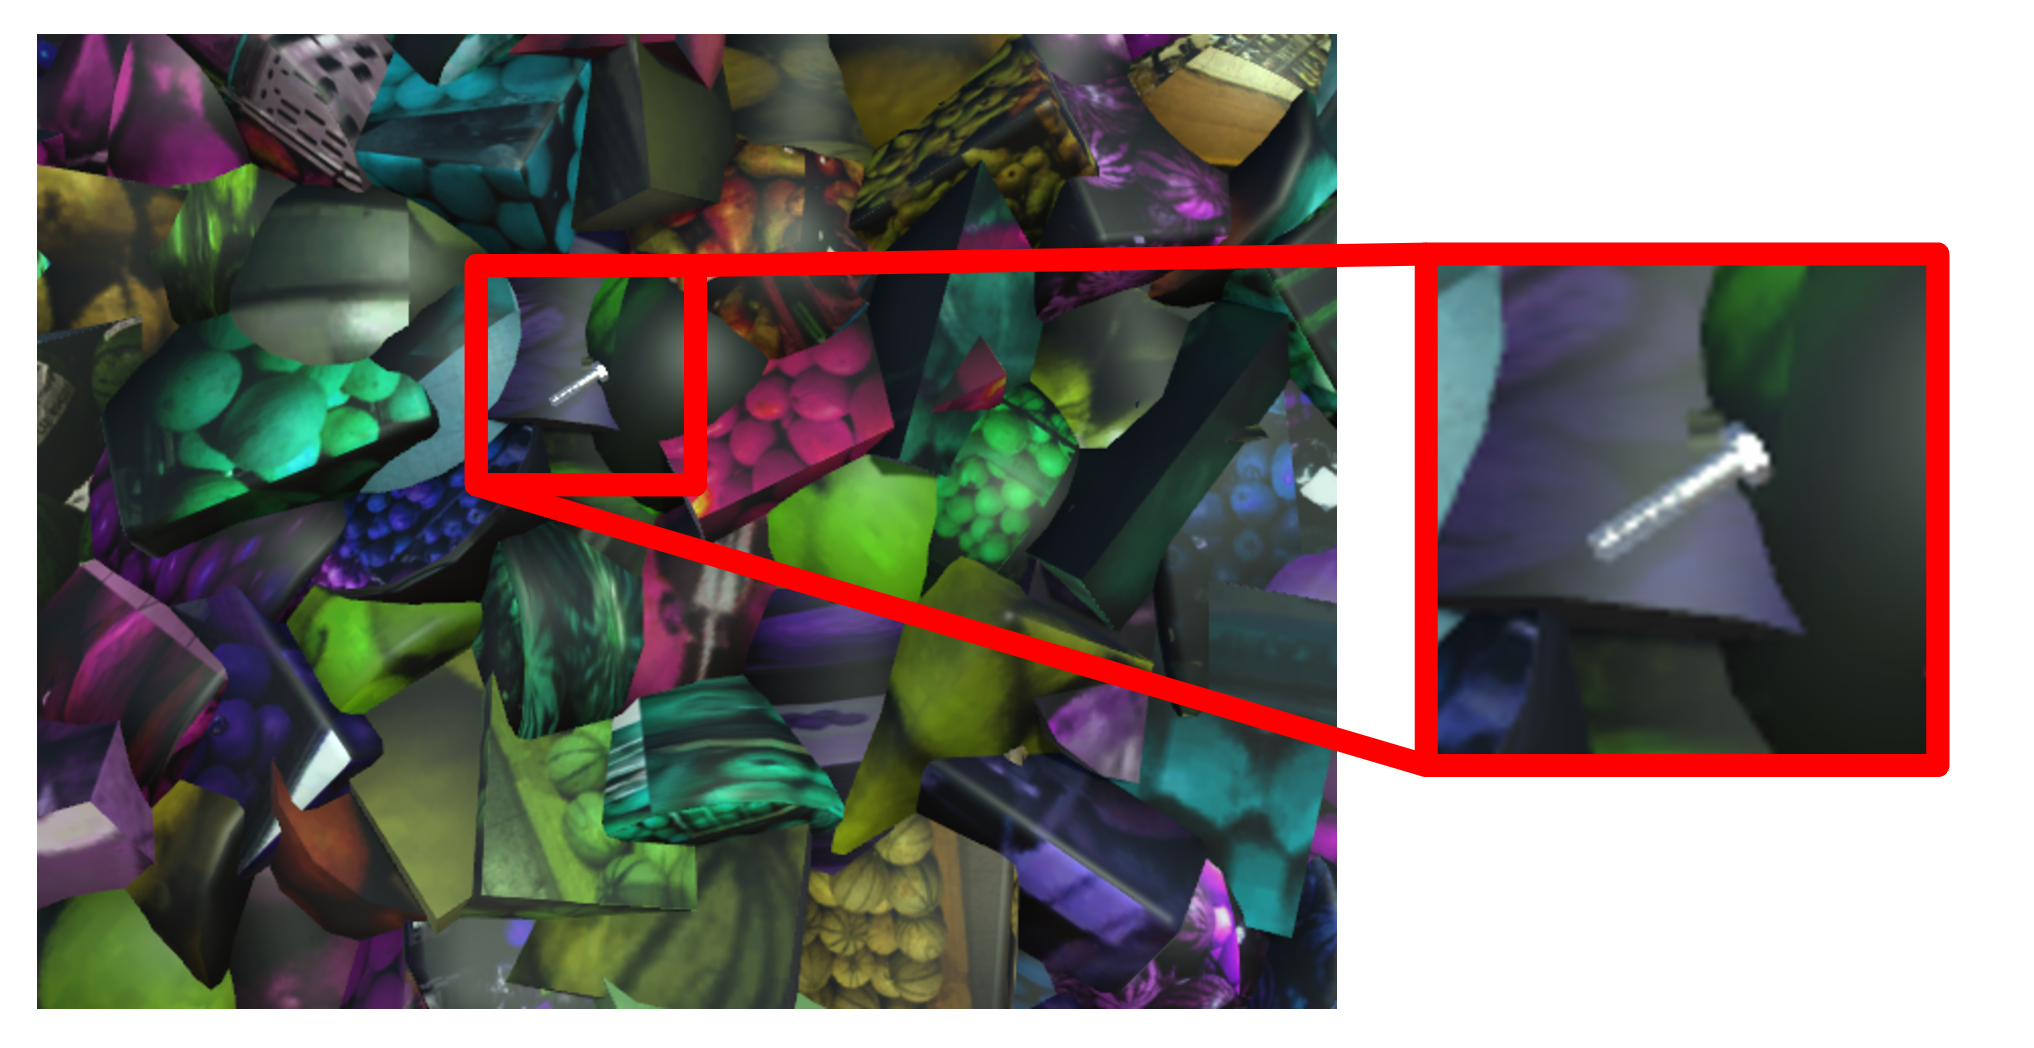
\includegraphics[width=0.6\textwidth]{screwdataset/ScrewDataset.png}
    \caption{One of the images generated with Unity's Perception package for training our model.}
    \label{fig:screwdataset}
\end{figure}

As a test case, we decided to generate a pose estimation dataset for a standard M6x30 hexagonal head screw. This is a very challenging object, as it is small and symmetrical. Symmetrical objects have always been difficult for pose estimation algorithms, due to reasons explained in depth in appendix 1. The model of the M6x30 screw was obtained from the FreeCAD Fasteners workbench\cite{Fasteners} and colored with a metallic texture.

The domain for this dataset consists of images of the screw placed inside of a scene: thus the primary domain variables are the pose, the background, and the lighting. We used a custom randomizer to set position and rotation for each iteration, and default randomizers provided as part of the Perception package to generate a background, composed by random 3D shapes placed with random positions, orientations and textures. Finally, we used a custom randomizer to set the lighting color, intensity and origin. A sample image from this dataset appears in figure \ref{fig:screwdataset}.

We can then interface the output of this procedure with EfficientPose using a conversion script, which performs the necessary tasks to make the dataset compatible with the generators used by the network. In this manner we can quickly and easily generate arbitrarily large datasets for training, by first running the Unity scenario, and then running the conversion script for EfficientPose.

\subsection{Training}

The original version of EfficientPose is trained on LINEMOD. However, the specifics of LINEMOD and of our own dataset are widely different: LINEMOD has around 1200 images per object, and only about 200 of these are used for training, while our dataset has 10000 images, 9000 of which are used for training. This means that we must set proper training parameters for our own dataset.

First, we reduced the number of epochs from 5000 to 100. Since our dataset contains 45 times more images, these two values represent a similar training time. EfficientPose also by default evaluates the model only every 10 epochs due to the small epoch size; we change this value to evaluate at the end of every epoch.

EfficientPose implements Keras' ReduceLRonPlateau callback to dynamically set the learning rate during training. This is standard practice: large learning rates quickly adjust the model but can lead to fluctuations, local minima and divergence; smaller learning rates avoid these issues but take an excessive amount of time to improve the model\cite{ReduceLR}. This method instead starts with a large learning rate, and then automatically reduces the learning rate whenever training stagnates, thus maintaining a value closer to the ideal. By default, EfficientPose halves the learning rate every time the accuracy does not improve for 25 epochs; we changed this to an 80\% reduction every 5 epochs, to account for the increased number of samples per epoch.

The initial and minimum learning rates are mantained identical to EfficientPose's, set at $10^{-4}$ and $10^{-7}$ respectively. For all purposes in this thesis, we will be using the networks scaled to their lowest hyperparameter $\phi = 0$, as going any higher requires inordinate amounts of time to train.

\section{Augmented Reality Datasets}

\subsection{Motivations and Objective}

In the previous section we explored the option of generating fully synthetic training images using domain randomization. This represents a "shotgun" approach: by representing a wide variety of environments and conditions in the dataset, we hope that the model learns to generalise to more situations, including eventually our usecase. However, this is only one way of bridging the reality gap. Another way could be to make this gap "smaller", by making the training images as similar as possible to the real environment the model will then be working in.

This approach has the disadvantage of fewer guarantees on performance outside of the selected environments, which makes it better for usecases which are stationary or limited to fewer settings. However, since we are considering applications in an industrial scenario, this is not really an issue for us.

To generate realistic images, we considered two options: either re-creating the environment inside the simulator, or using an "augmented reality" approach by rendering the 3D models of the dataset objects on top of real photographed images taken from the testing environment. We decided on the second option, since it is both faster and gives more realistic final results compared to a fully simulated environment.

Thus our objective is to create a method to easily and quickly generate a realistic training dataset for our testing environment, which is a simple table with a set of objects placed on its surface.

\subsection{Generation Methodology}

We again use Unity Perception to generate our training dataset, as described in \ref{ss:ScrewDataset}. We used models for 5 objects: the same M6x30 screw used previously, a M8x16 round head screw, a M8x25 and M8x50 socket head screws, and a M4x40 countersunk screw. As previously stated, these are small, symmetric objects that are generally challenging to identify, with the additional complication that they all have similar shapes and sizes. Only the first four are annotated, while the M4x40 is included as a "decoy" to reduce the number of false positives (further explained in subsection \ref{false_positives_issue}).

The key issue now becomes the positioning of the objects in the image. Since in real-life conditions, the pose of an item is almost always influenced to some degree by its environment, we believe that simply placing the item freely in 6D space as we did in the previous approach would lose information compared to a realistic placement. Taking our example setting where the objects are placed on a surface, this constrains three degrees of freedom for each object: the vertical position relative to the surface, and the two rotations around the axises that determine the surface itself. Thus our objective is, for each background image, to start from the pose of the surface relative to the camera, and from there generate a realistic pose for each dataset object, so that the object appears to be placed on the surface.

This pose is generated using the composition in sequence of three roto-translations:

\begin{enumerate}
    \item An initial transformation $(t_s, \text{R}_s)$ from the camera frame to the surface's reference frame.
    \item A second transformation $(t_r, \text{R}_r)$ that shifts the object from the surface frame to a random position and rotation.
    \item A final correcting transformation $(t_c, \text{R}_c)$ that takes into consideration the object's geometry to obtain a realistic placement.
\end{enumerate}

\begin{figure}[ht]
    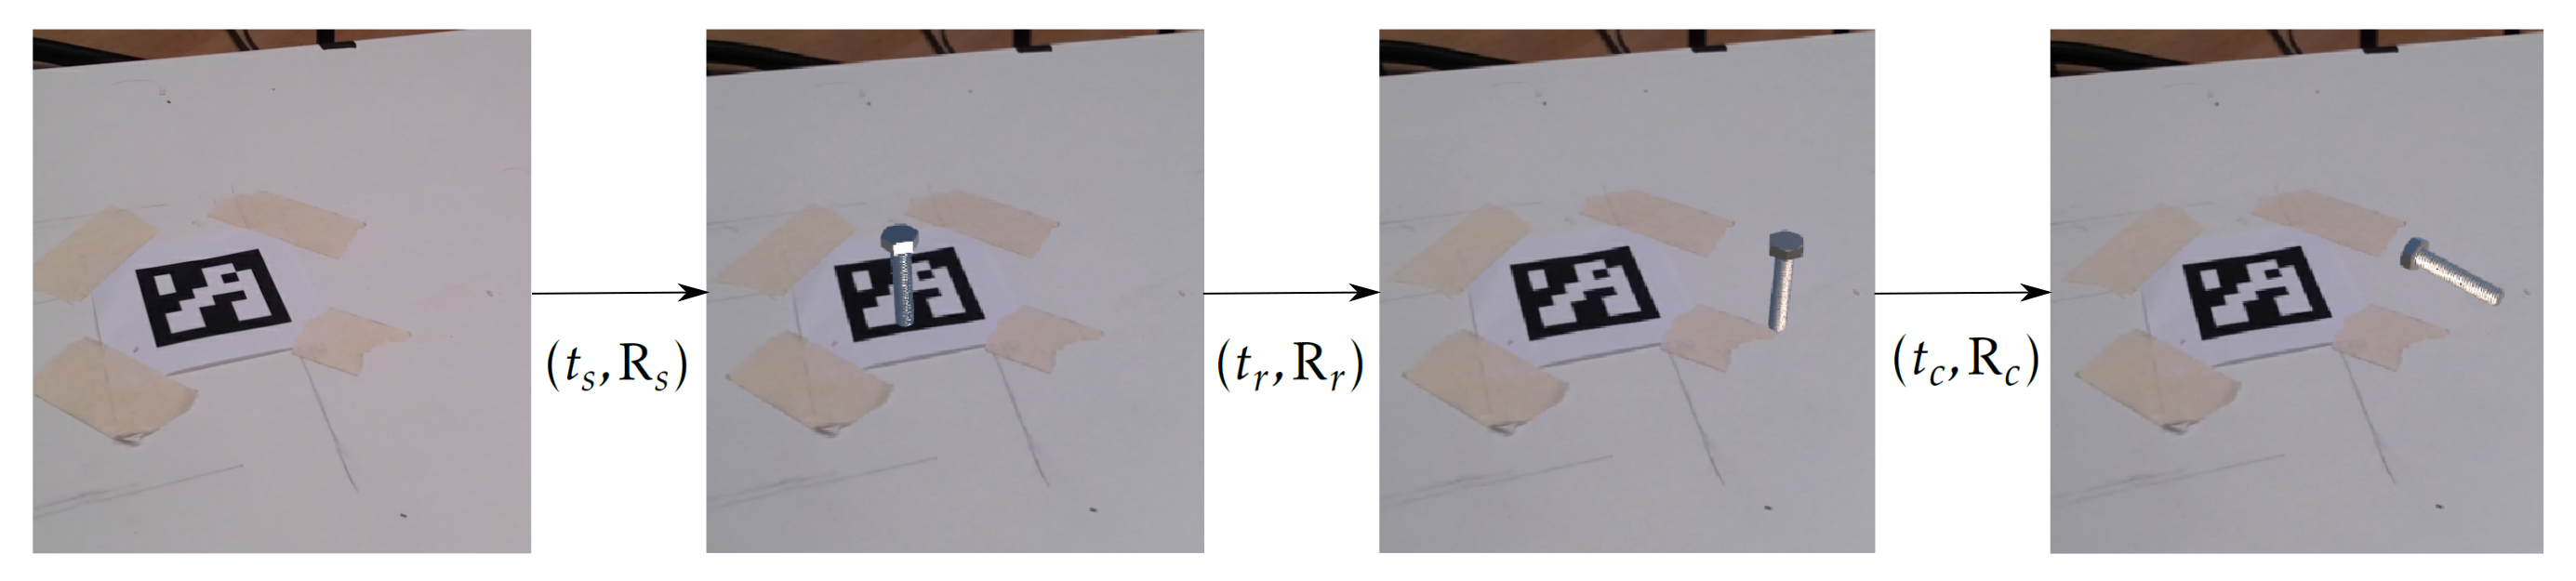
\includegraphics[width=\textwidth]{movement_phases.png}
    \caption{Visualization of the three roto-translations used to obtain a realistic placement.}
\end{figure}

We can obtain the initial transformation $(t_s, \text{R}_s)$ by preparing the testing surface with an ArUco marker. In this manner, by capturing a video of the surface, eliminating off-center and blurry frames, and undistorting the resulting images, we obtain backgrounds for our scene that are then associated with the pose of the marker, as previously described in section \ref*{s:notlearningbasedmethods}.

We then compute values of $t_r$ and $\text{R}_r$ considering the degrees of freedom afforded to each object by the surface: that it is free to translate along the surface's x and y axes, and to rotate around its z axis.

\begin{equation*}
    t_r = 
    \begin{bmatrix}
        x_r\\y_r\\0
    \end{bmatrix}
    ,\; \; \text{R}_r =
    \begin{bmatrix}
        \cos \theta_r & - \sin \theta_r & 0 \\
        \sin \theta_r & cos \theta_r & 0 \\
        0 & 0 & 1
    \end{bmatrix}
\end{equation*}

$x_r$, $y_r$, and  $\theta_r$ can be extracted from pre-defined probability distributions; in our case three uniform distributions $U(x_{min}$, $x_{max})$, $U(y_{min}, y_{max})$, and $U(\theta_{min}, \theta_{max})$.

The final correction transformation $(t_c, \text{R}_c)$ differs based on the object geometry, thus must be computed individually for each object. For example, if we consider the M6x30 screw, $(t_c, \text{R}_c)$ is given by a translation $z_c$ along the z-axis and a rotation by $\theta_c$ around the y-axis:

\begin{equation*}
    t_c = 
    \begin{bmatrix}
        0\\0\\z_c
    \end{bmatrix}
    ,\; \; \text{R}_c =
    \begin{bmatrix}
        \cos \theta_c & 0 & -\sin \theta_c\\
        0 & 1 & 0\\
        \sin \theta_c & 0 &  \cos \theta_c
    \end{bmatrix}
\end{equation*}

The resulting transformation is shown in figure \ref*{fig:screwdim}, while $z_c$ and $\theta_c$ depend on the dimensions of the screw as follows:

\begin{figure}[ht]
    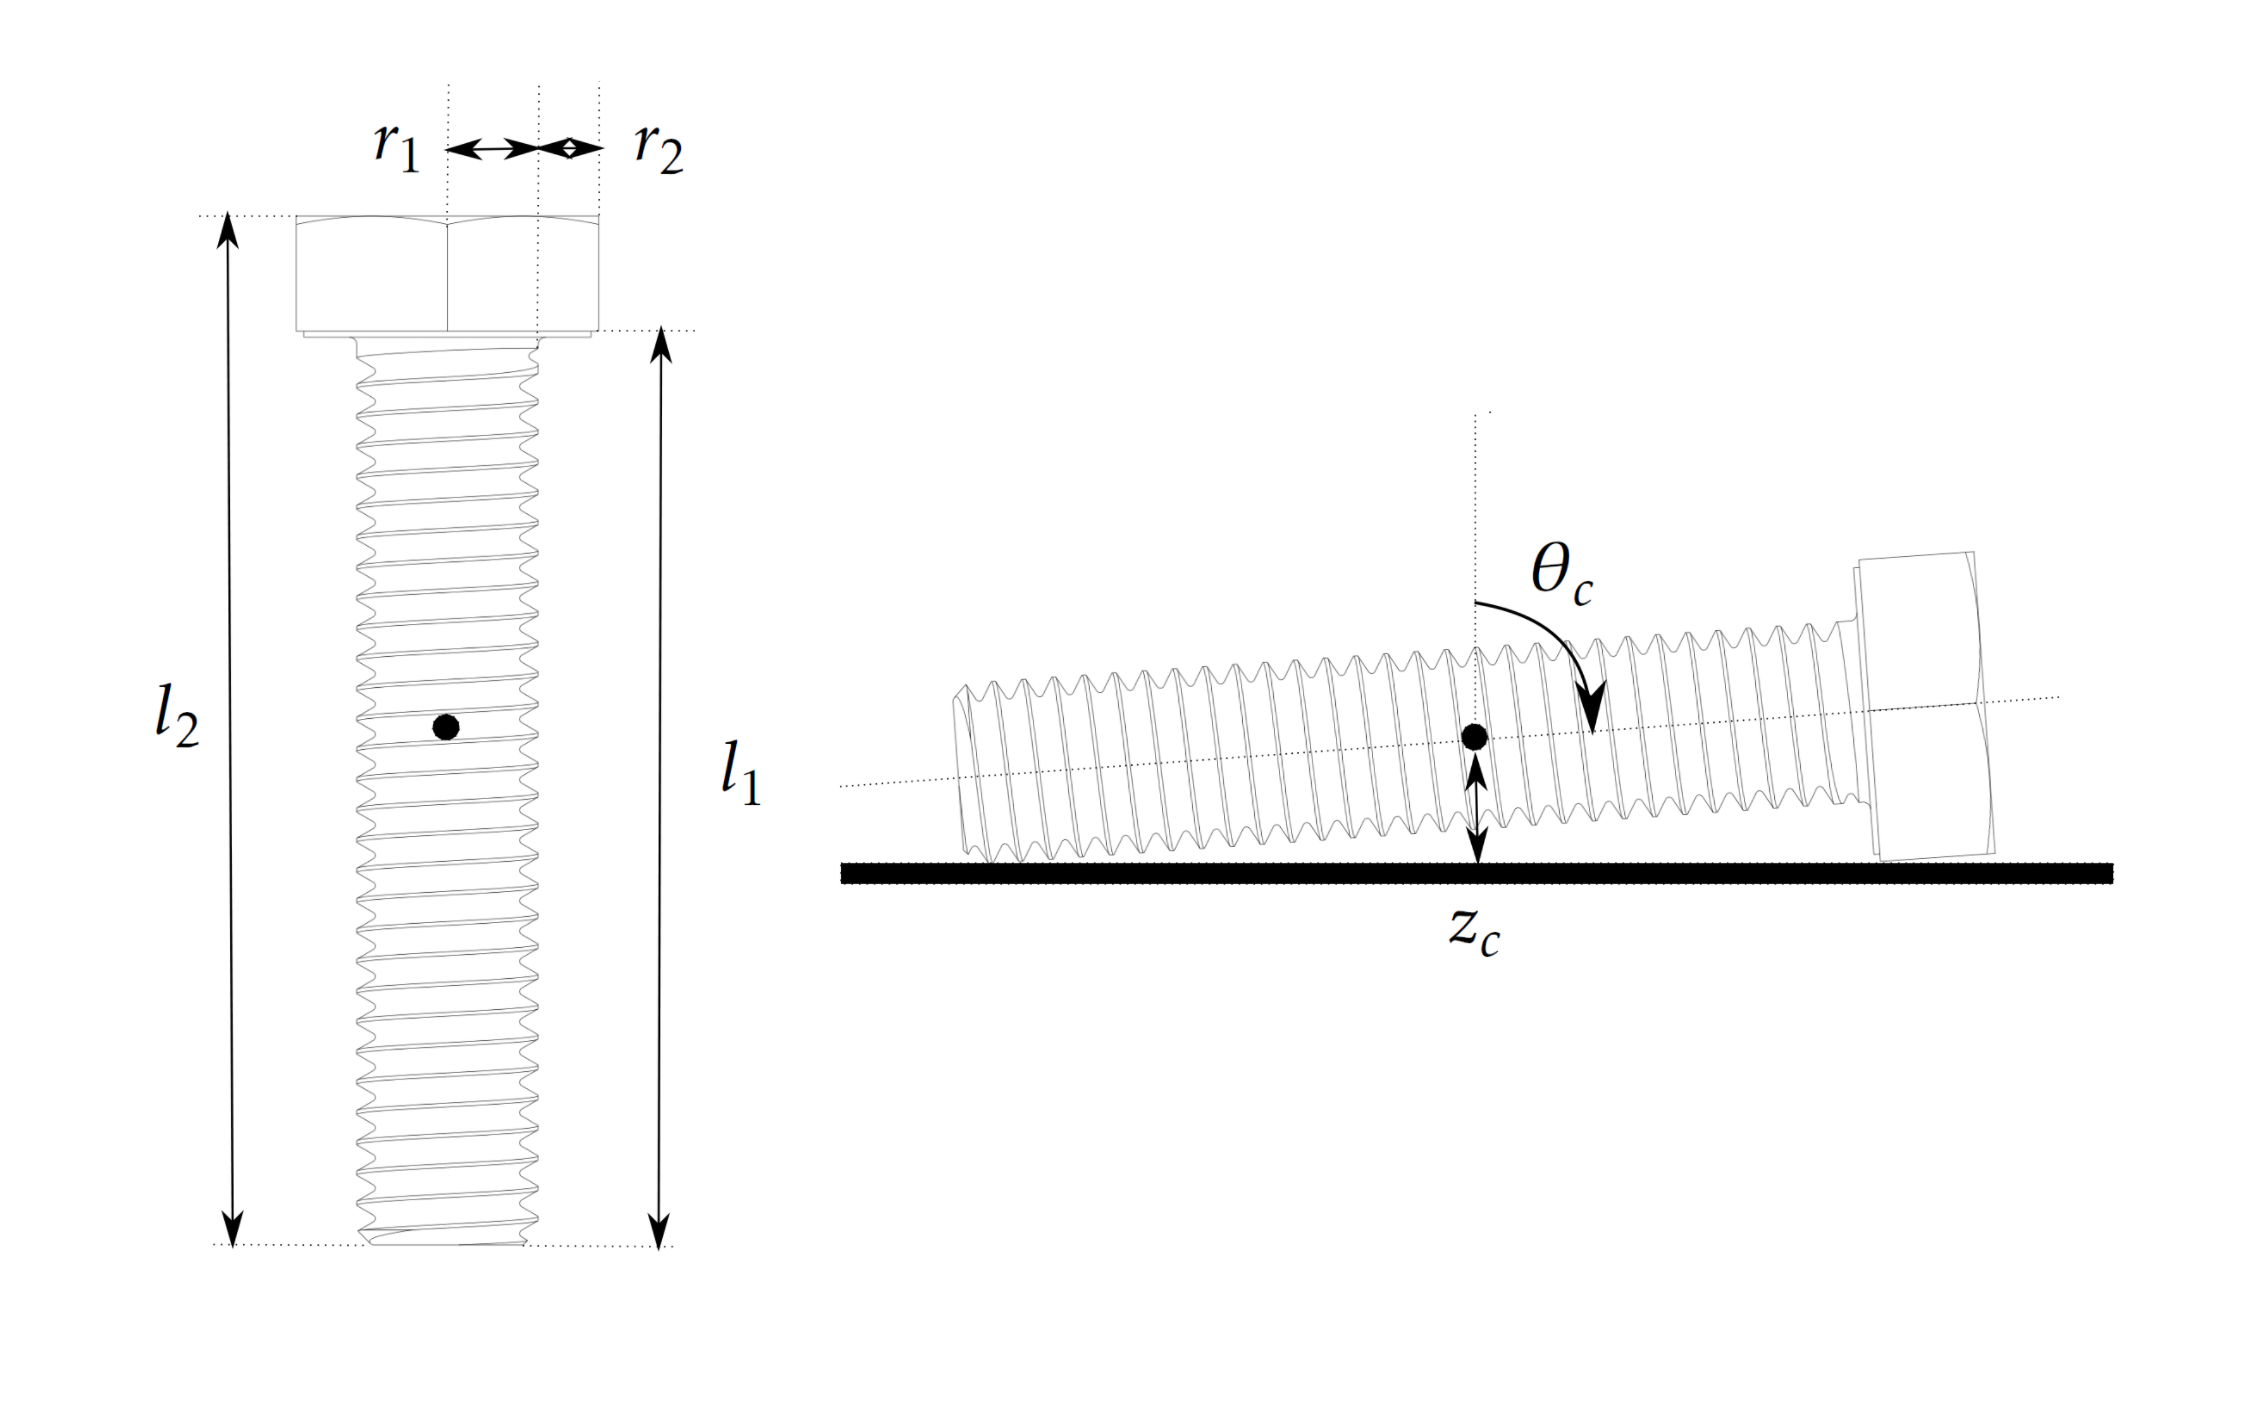
\includegraphics[width=0.8\textwidth]{screwdims.png}
    \caption{Dimensions and pose corrections for the M6x30 hexagonal head screw.}
    \label{fig:screwdim}
\end{figure}

\begin{align*}
    \theta_c &= \frac{\pi}{2} - \arctan \frac{r_2}{l_1}\\
    z_c &= r_1 \sin \theta_c + \frac{1}{2} l_2 \cos \theta_c
\end{align*}

One thing to note is that if an object can have multiple positions on the surface, we consequently have multiple correction transformations to choose from. For example, each screw could be on its side or on its head, which implies a choice between two sets of $t_c$, $R_c$.

Once we have the three transformations $(t_s, \text{R}_s)$, $(t_r, \text{R}_r)$ and $(t_c, \text{R}_c)$, the final pose $(t, \text{R})$ in camera reference is computed as:

\begin{align*}
    t &= t_s + \text{R}_s t_r + \text{R}_s \text{R}_r t_c\\
    \text{R} &= \text{R}_s \text{R}_r \text{R}_c
\end{align*}

Eventual intersections between objects resulting from successive placements are resolved using a simple brute-force approach: whenever a placement would generate a collision, the process is re-attempted from the second step, with a limit on the maximum number of attempts allowed.

With this method, for each background we can quickly generate a series of training images with associated ground truths. While we considered the particular situation of a set of objects placed on a flat surface, the three steps of this approach can be applied to other conditions. In general, these steps are:

\begin{enumerate}
    \item The identification of the area of interest, and primary placement inside that area.
    \item A random transformation within the area of interest, dictated by the degrees of freedom present.
    \item A final transformation dictated by the specifics of the object to be placed.
\end{enumerate}

\subsection{Data Augmentation and Training}

\begin{figure}[ht]
    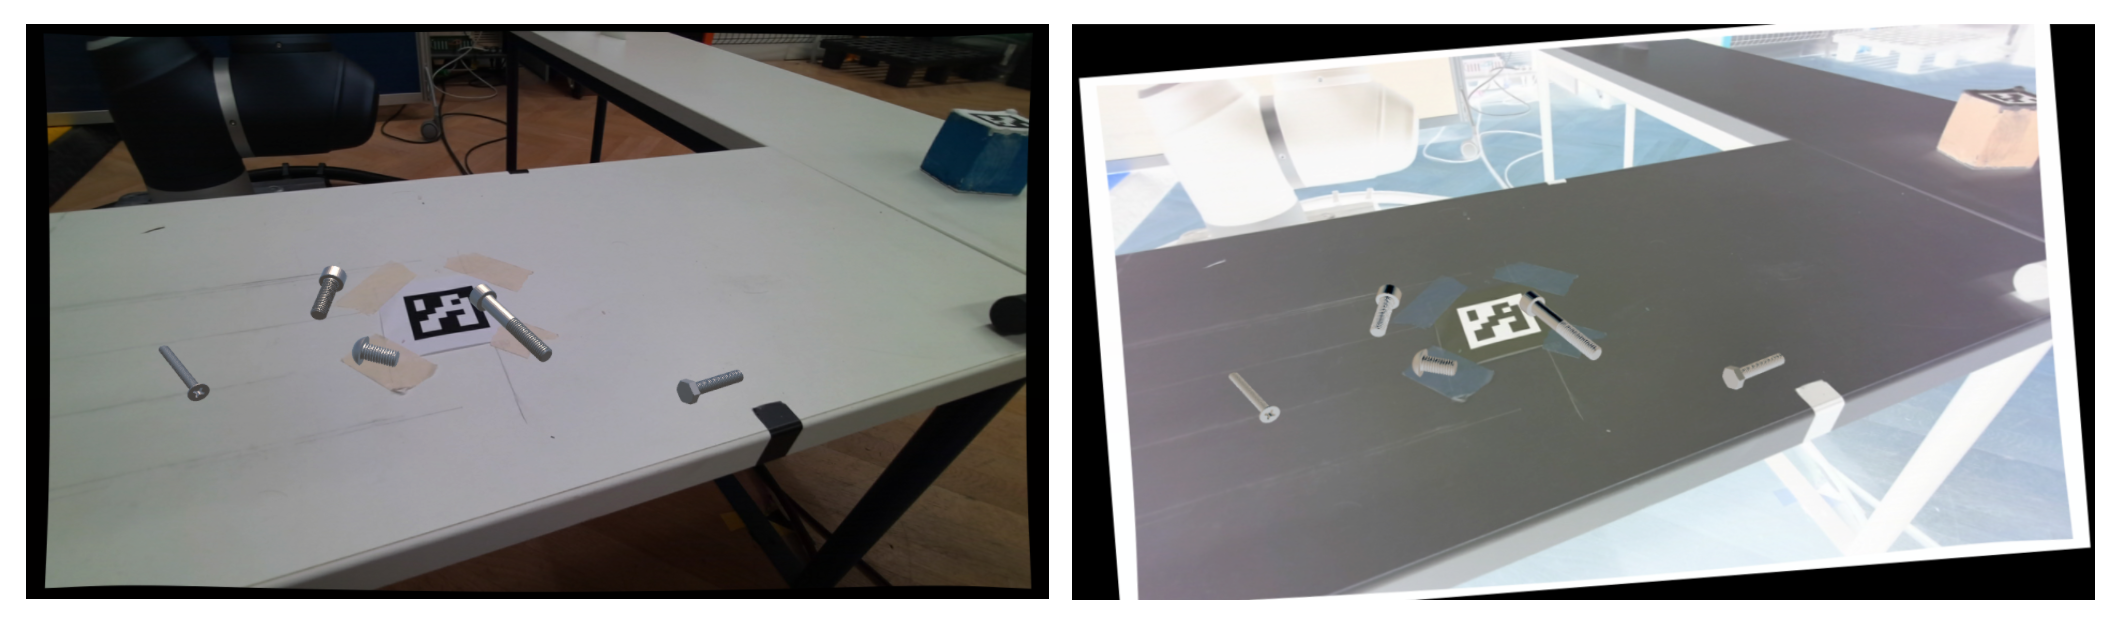
\includegraphics[width=\textwidth]{screwposeaugmented.png}
    \caption{An example of a training image before and after data augmentation.}
    \label{fig:ScrewPoseAugmented}
\end{figure}

The dataset generated with the previous methodology has two major weaknesses. First, there is a limited number of background images, which means that the model has a finite number of camera positions to learn from. This may lead to overfitting and unreliable results for positions that don't have sufficient representation. Second, it is difficult to randomize light intensity and color for the background images inside Unity, as it is decoupled from the 3D models.

We can remedy these issues using data augmentation. This is a technique that involves applying random changes to data during training, similarly to how domain randomization would apply during dataset generation. EfficientPose already provides two data augmentation methods: 6 Degree-of-Freedom augmentation and color augmentation. 6 Degree-of-Freedom augmentation involves randomly rescaling and rotating the input image and consequently adjusting the ground truth, so as to greatly increase the number of possible poses each image can provide. Color augumentation instead implements RandAugment\cite{RandAugment} to change the color and grain for the entire image. Applying both these methods results in images such as the one depicted in figure \ref{fig:ScrewPoseAugmented}, conveniently fixing the issues of our dataset.

Other training parameters are identical to the previous attempt with the fully synthetic dataset: 100 epochs, with an 80\% learning rate reduction if the model stagnates for 5 epochs.

\section{Semantics Applications}

\subsection{Motivations and Objective}

In many applications, it may be that estimating the pose of an object is sufficient to perform the task. However, it it often necessary to infer additional information from this data. A typical situation is the assembly of a workpiece from its components, where while tracking the pose of each individual component we may also have to track the state of the assembly itself.

Thus we want to ascertain if it is viable to use pose estimation techniques to track the position of the components for an assembly task, and simultaneously obtain information of its overall state.

\subsection{Dataset Generation and Training}

The first step to working with neural networks is again the generation of the datasets required for training and evaluation. For our task, we are considering the assembly of a set of modular button boards. We have two boards, one with two slots, and one with three slots. These slots can be filled in any order with one of three buttons: a larger safety button, and two smaller buttons with different designs on their faces, but identical shape. The CAD models for these objects were available online from the supplier's website, and we used Blender to color them appropriately. Renders for these objects are depicted in figure \ref{fig:buttonpose_objects}.

\begin{figure}[ht]
    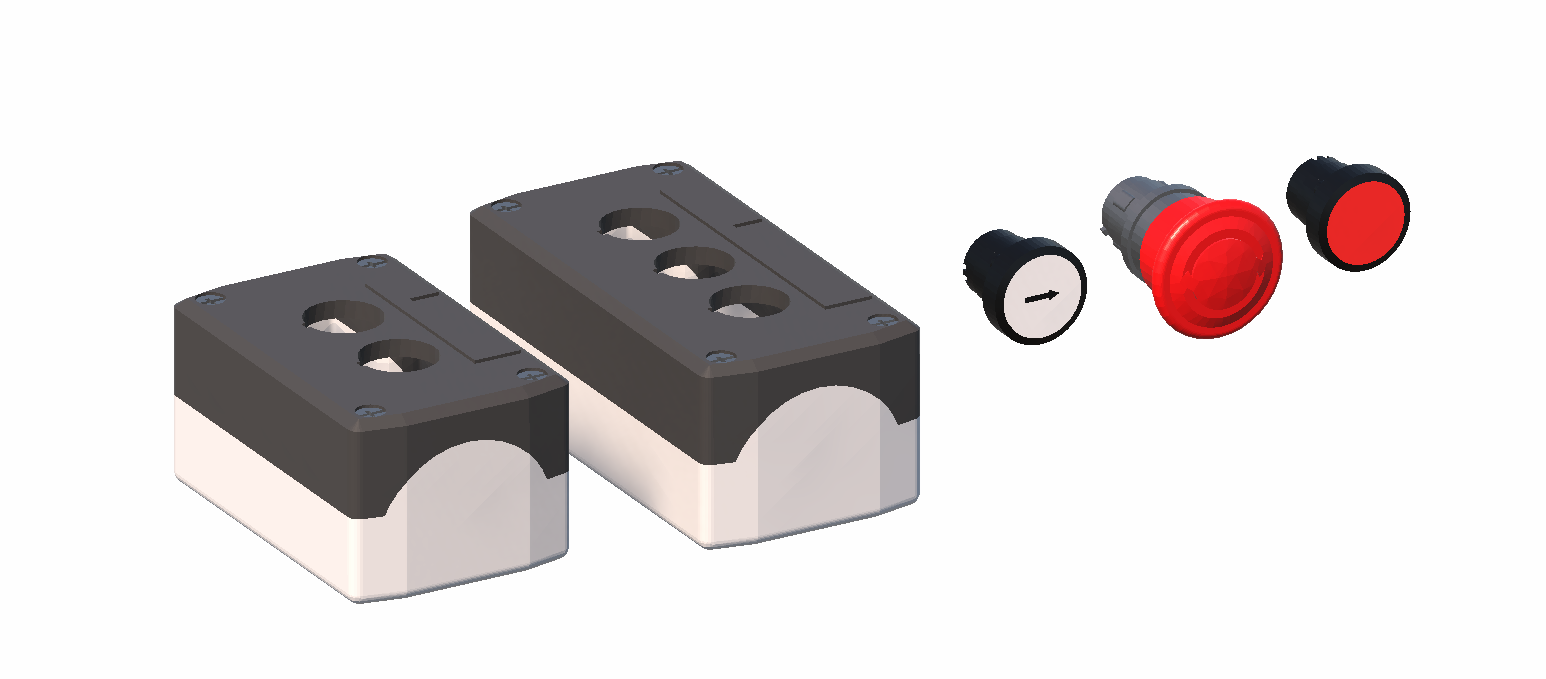
\includegraphics[width=0.6\textwidth]{buttonpose_objects.png}
    \caption{Orthographic rendering of dataset objects: two modular button boards and three buttons.}
    \label{fig:buttonpose_objects}
\end{figure}

To generate the dataset images we exploited the previously mentioned Augmented Reality method, however we have a few noticeable differences that require consideration. The first obvious one is that we would like to represent the buttons not only while they are freely placed on the table surface, but also when they are slotted into a board. This is achievable by positioning the button with the same pose as the board, and then applying a final roto-translation that shifts the button into a slot. We can compute these transformations in advance and simply apply them when necessary.

One important thing to note is that these roto-translations depend on the shape of the button: thus the safety button will require different values compared to the other two.

The second, issue deals with the two smallet buttons with identical shape. These buttons are distinguishable only by the different designs on their faces, but when placing them randomly, there is a good chance that these faces are not visible. This leads to a situations where it is impossible to differentiate between the two, causing a drastic drop in performance, as during training the network will percieve a large number of false positives.

To solve this issue, we can add a fictional object to the dataset, the "unidentified button". Simply put, we categorize buttons without their unique face visible as a new object class, since it is impossible for the network to directly identify them as one type or the other.

\begin{figure}[ht]
    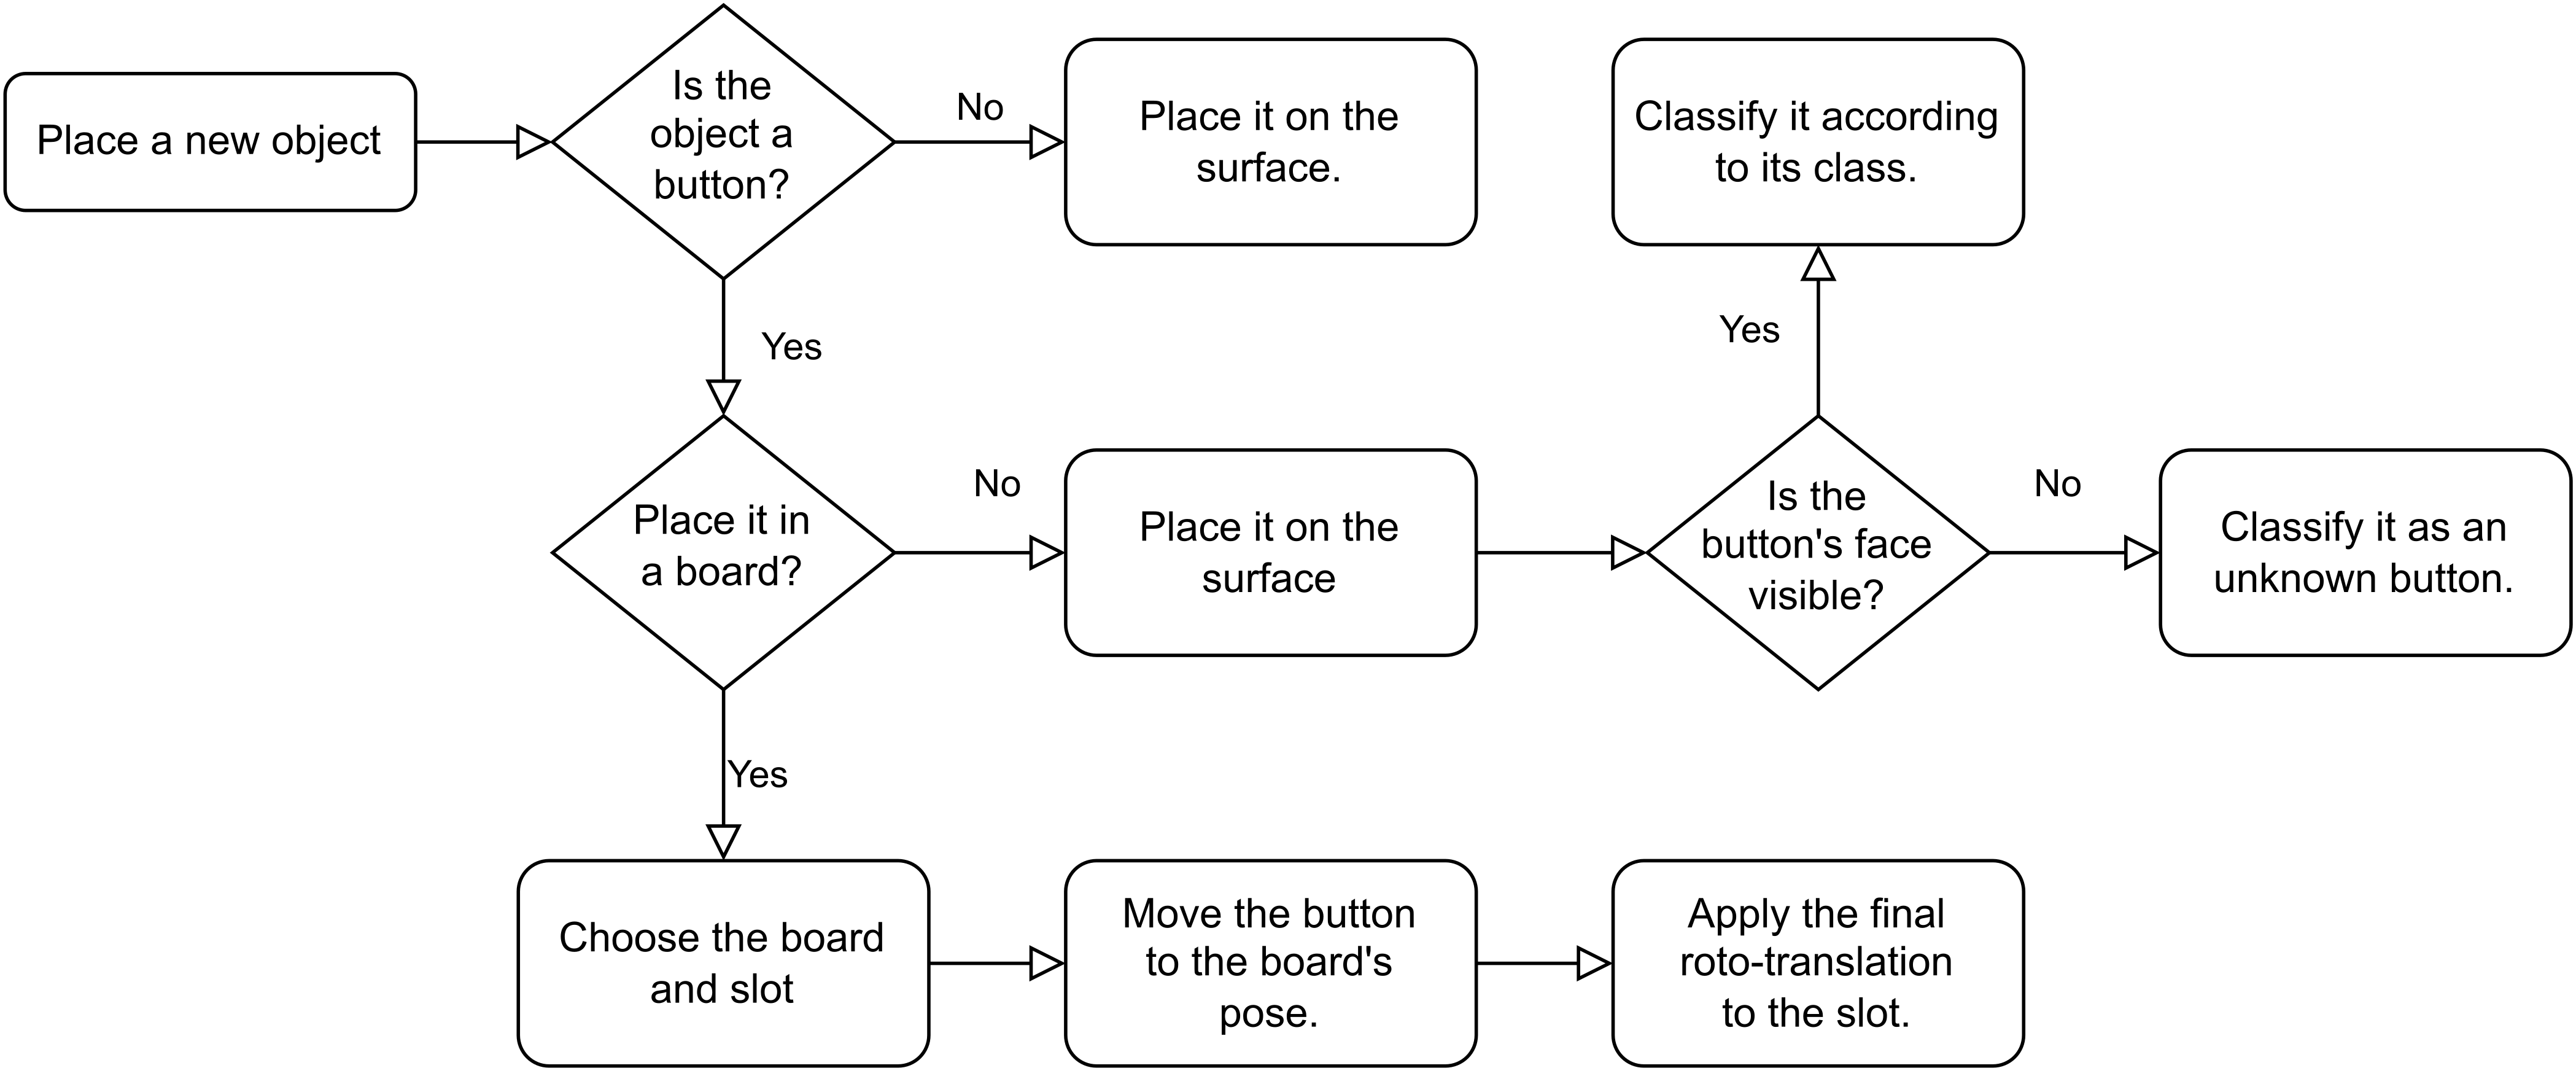
\includegraphics[width=\textwidth]{buttonpose_placement.png}
    \caption{Flowchart representing the algorithm for placement of dataset objects, when placing buttons inside of slots and checking for face occlusion.}
    \label{fig:buttonpose_placement}
\end{figure}

We can use a simple geometric method to determine if a button's face is visible during generation, explicated in figure \ref{fig:button_occlusion}. Considering the origin of the camera reference frame $O = [0, 0, 0]^T$, the button's pose is given by the translation vector $t$ and the rotation matrix R. $t$ also indicates the position of the center of the button $C$, due to it being the origin of the button's 3D model. If we then consider the vector $f = [f_x, f_y, f_z]^T$ indicating the position of the center of the button's face $F$ in the button's frame of reference, the position of this point in the camera frame is given by:

\begin{figure}
    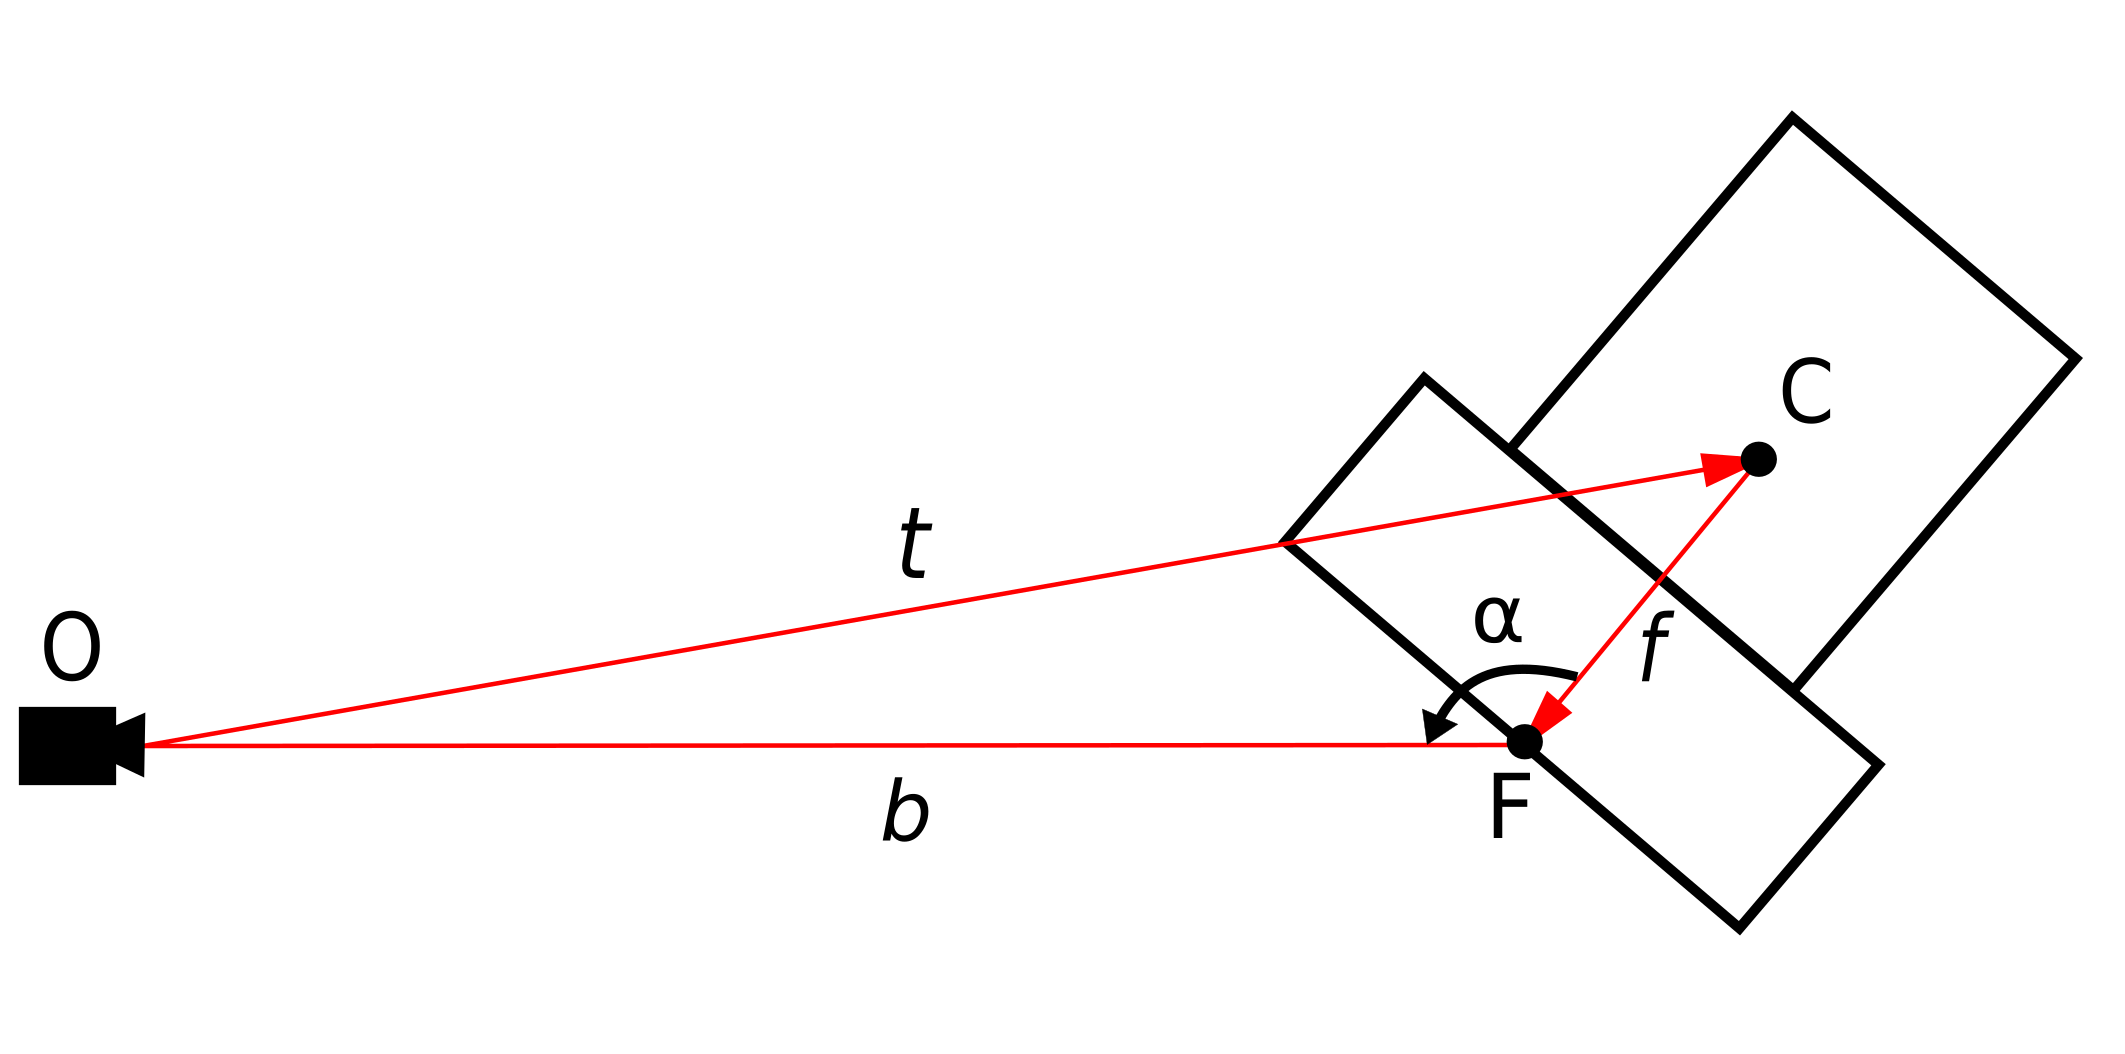
\includegraphics[width=0.7\textwidth]{button_occlusion.png}
    \caption{Schematic representation of the button relative to the camera, and of the variables used when evaluating occlusion of the button face.}
    \label{fig:button_occlusion}
\end{figure}

\begin{equation*}
    F = t + \text{R}f
\end{equation*}

We can then compute the amplitude of the angle $\alpha = C\hat{F}O$. Denoting $OF=b$, we apply the law of cosines:

\begin{equation*}
    t^Tt = b^Tb + f^Tf -  2||b||\cdot ||f|| \cdot \cos \alpha
\end{equation*}

By making $\alpha$ explicit in this equation we obtain:

\begin{equation*}
    \alpha = \cos^{-1}\left(\frac{t^Tt- b^Tb-f^Tf}{2||b||\cdot||f||}\right)
\end{equation*}

It is simple to verify geometrically that the button's face is occluded whenever $\alpha < 90\degree$, and viceversa. To avoid strange edge cases where the button's face is barely visible in the proximity of $\alpha = 90\degree$, we introduce a small buffer angle $\beta$, usually around 5\degree. Thus we categorize a button as unrecognizeable whenever $\alpha < 90\degree + \beta$, overwriting its class in the ground truths with the "unknown button" class.

We decided to generate 20'000 images in this manner, where 18'000 are used for training and 2'000 for verification. The increased datset size is due to us giving the required representation to each of the unique positions each object can have. We subsequently reduced the number of epochs to 40, and the patience for learning rate reduction to 3 epochs. All other parameters are identical to our previous attempts.

\subsection{Semantic Meaning Extraction}

Now that we have a dataset and a model trained on it, we can begin the task of creating a method to identify the state of the overall assembly. There are two pieces to this assembly: buttons and the boards they're to be slotted in. The problem now becomes: given the position of a button and the position of a board, how does one determine whether the button is slotted into the board, and in which slot?

We handle this using an intuitive three step method:
\begin{enumerate}
    \item For each button and slot, we compute a \emph{distance metric} that represents the button's "distance" from that slot.
    \item We compare this metric with a \emph{distance threshold}: if it is less than this value, the button is considered a viable candidate for filling the slot.
    \item We resolve conflicts between multiple buttons competing for the same slot and vice-versa.
\end{enumerate}

For \emph{distance metrics}, we considered two possible candidates: Center-to-Center distance and Average Symmetric Distance.

\begin{figure}[ht]
    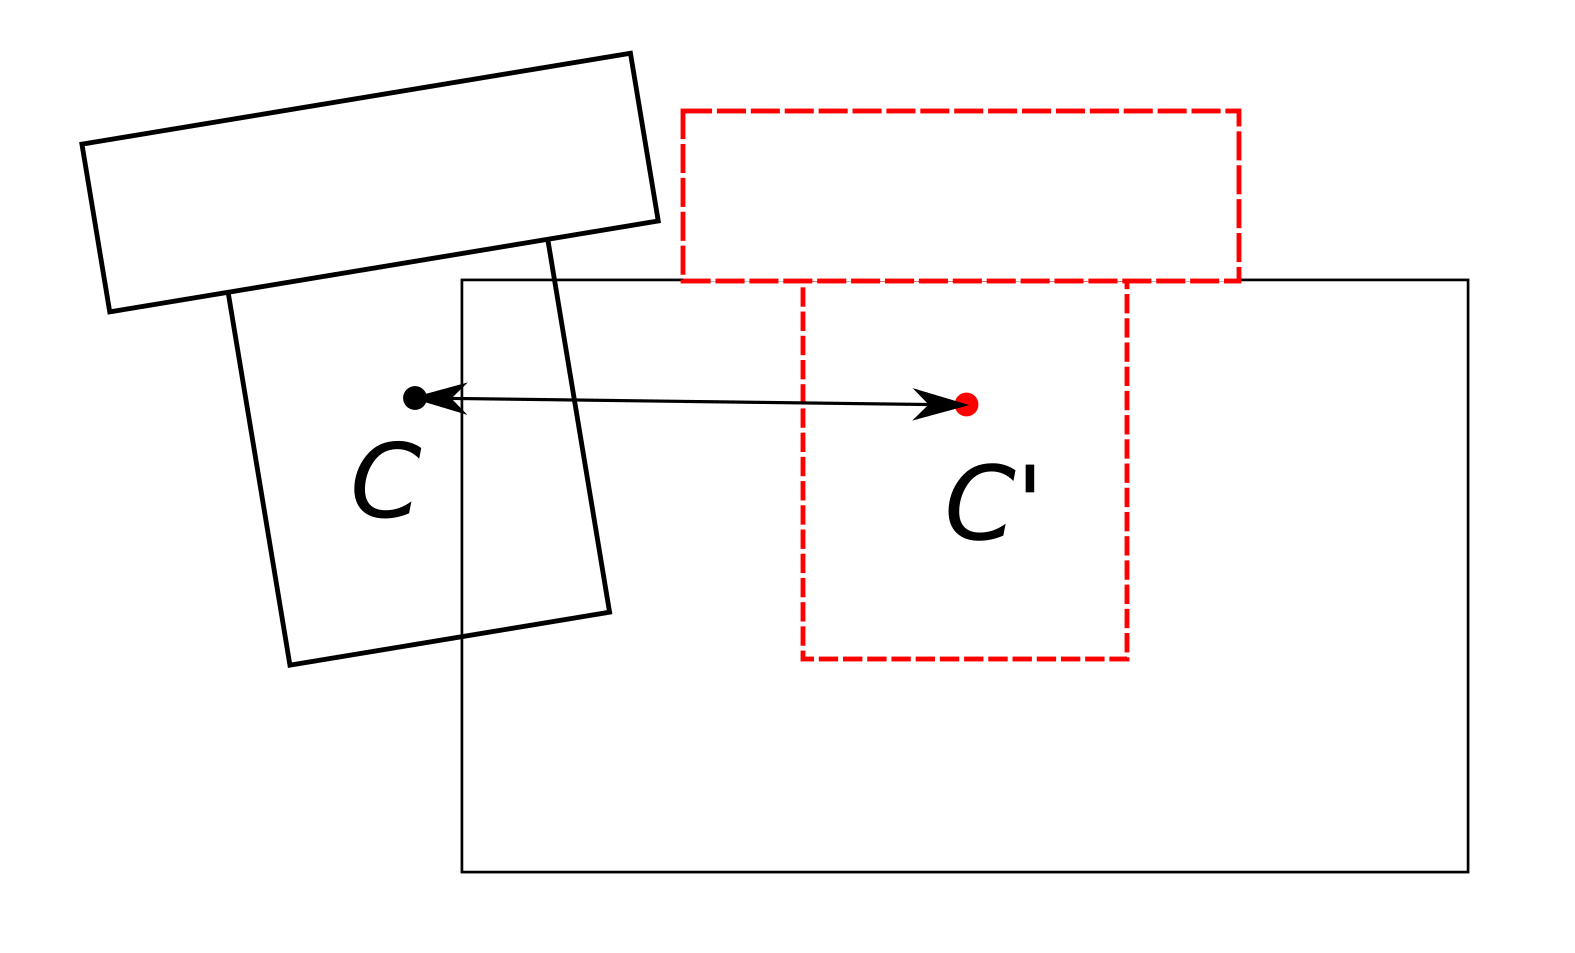
\includegraphics[width=0.6\textwidth]{Center-to-center.png}
    \caption{Depiction of the center-to-center distance from a button to a slot. In black is the estimated pose of the button, while in red is the estimated position of a button if it was hypothetically already in the slot.}
    \label{fig:center2center}
\end{figure}

Center-to-Center is the distance between the estimated position of the center of the button $C$, and the position this center would have if the button was already in the slot, $C'$, as depicted in figure \ref{fig:center2center}. While the first position is a direct output of our network, the second one must be obtained from the succession of three roto-translations: one from the camera reference to the estimated position of the board, which is a direct output of the network; a second to the position of the slot relative to the board, which is known for each slot; and the last one from the position of the slot to the position of the hypothetical button center, which varies based on the geometry of the button. The Center-to-Center distance is then given by $||CC'||_2$.

The Average Symmetric Distance is instead identical to the AD-S computed as a metric during training and evaluation. Considering again the estimated pose of the button $(\text{R}, t)$ and the pose the button would have if it was considered in the slot $(\text{R}', t')$, the average distance is computed as:

\begin{equation*}
    \text{AD-S} = \frac{1}{n} \sum_{x_1 \in M} \min_{x_2 \in M} ||(\text{R}x_2 + \text{t}) - 
    (\text{R}'x_1 + \text{t}')||_2
\end{equation*}

where M is the set of the points composing the button's 3D model, and n is the number of points considered. While this metric has the advantage of considering differences in rotation, which Center-to-Center is unable to do, it is also much more demanding computationally, depending on the number of points considered.

Once we have a \emph{distance metric}, it is necessary to develop a conflict resolution algorithm. This is of fundamental importance for higher values of the threshold, since multiple slots will be within range of the same button or multiple buttons will be in range of the same slot, as depicted in figure \ref{fig:conflicts}.

\begin{figure}[ht]
    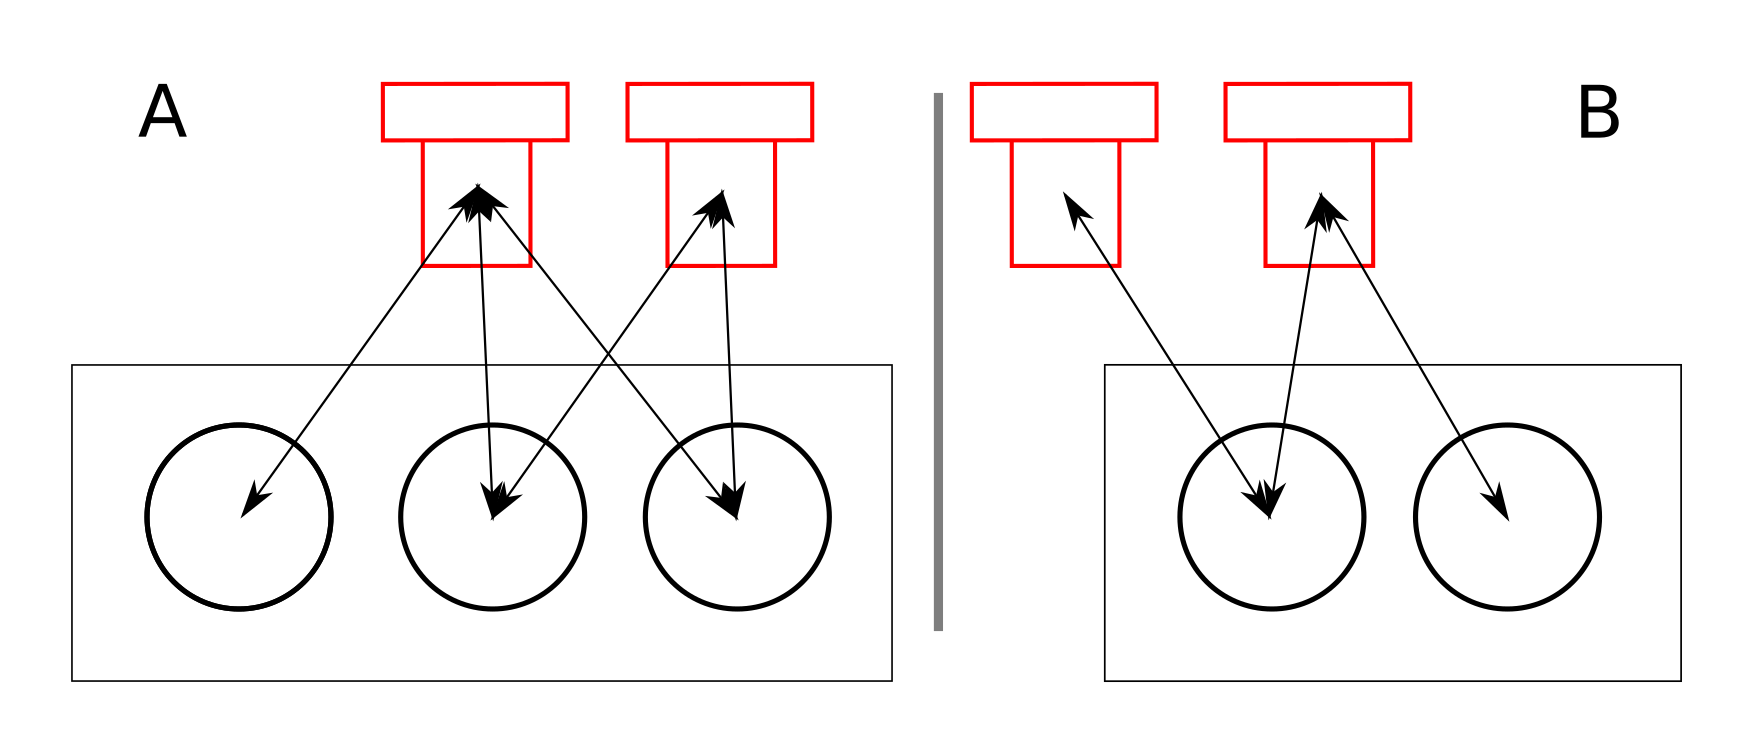
\includegraphics[width=0.8\textwidth]{buttons_conflict.png}
    \caption{Schematic depiction of two hypothetical situations that would generate conflicts by placing multiple buttons within the threshold of a single slot or vice-versa.}
    \label{fig:conflicts}
\end{figure}

For this purpose we introduce a "double check" method that provides excellent results with minimal complexity. This method is composed of three steps:

\begin{enumerate}
    \item For each button, we assign it to the closest slot within the threshold, if there is one.
    \item For each slot, we assign it to the closest button within the threshold, if there is one.
    \item For each assignment, it is confirmed only if it is reciprocated, and otherwise it is ignored.
\end{enumerate}

An assignment from a slot to a button is considrered reciprocated only if the button is also assigned to the slot, and vice-versa.

\begin{figure}[ht]
    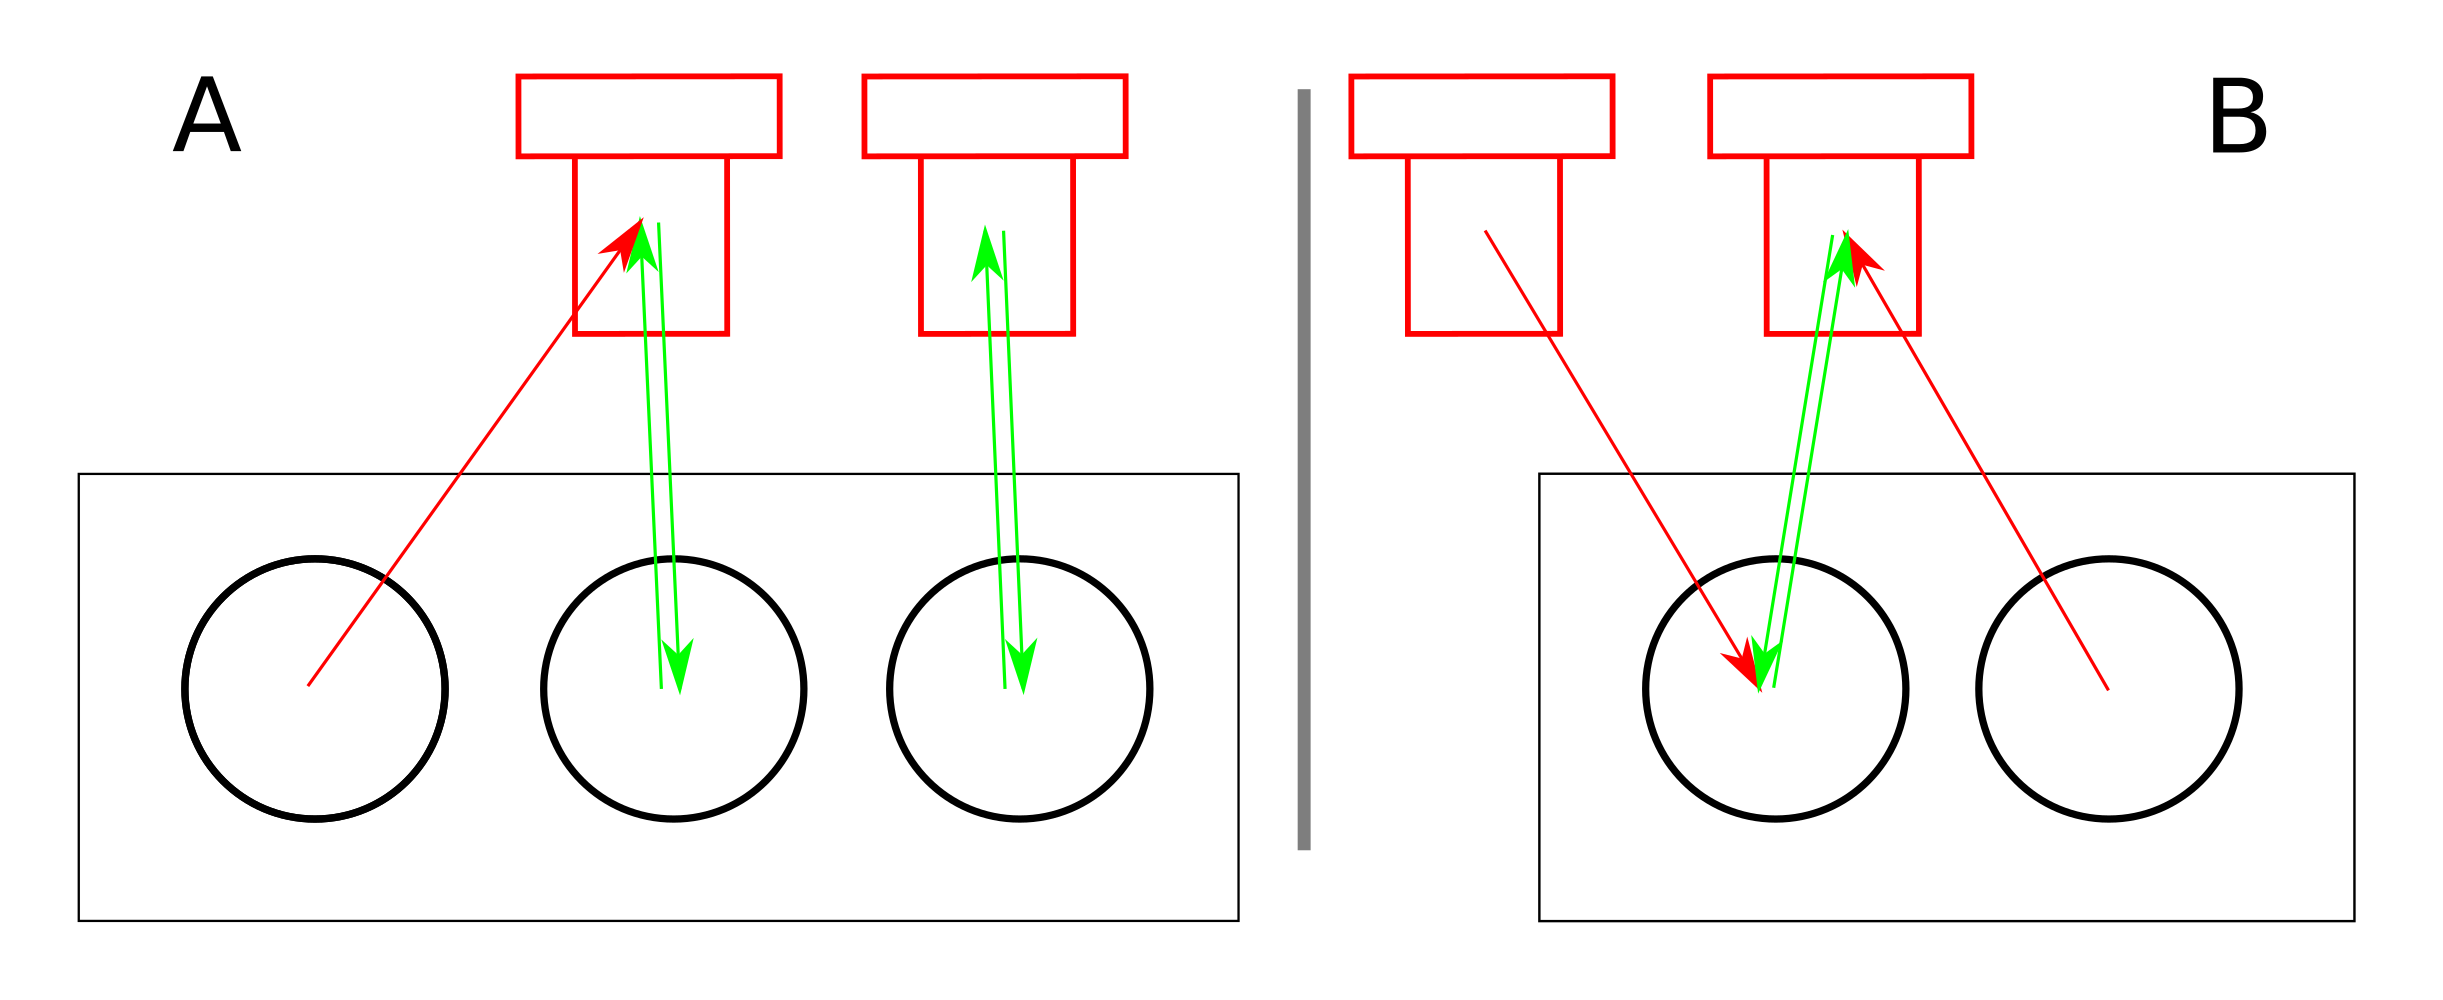
\includegraphics[width=0.8\textwidth]{buttons_resolution.png}
    \caption{Schematic depiction of the resolution of the conflicts previously depicted in figure \ref{fig:conflicts}. Green arrows represent reciprocating assignments, which are confirmed, while red arrows represent non-reciprocating assignments, which are ignored.}
    \label{fig:resolution}
\end{figure}

In this way we can resolve most possible ambiguites that may result during evaluation of the semantic state.

